\section{Физико-химические свойства пластовых флюидов}

Для расчёта свойств флюидов в \unf{} используется модель нелетучей нефти (black oil model). Это простая модель, в которой предполагается наличие в нефти только двух фаз -- жидкости и газа. Модель позволят рассчитать параметры флюидов, наиболее сильно влияющие на свойства потока - плотности фаз, вязкости и их объёмные соотношения в зависимости от давления и температуры.

В модели задания свойств флюидов \unf{} выделяются два набора свойств.
\begin{itemize}

\item Статичные свойства флюида (\mintinline{vb.net}{PVT_prop}) - плотность нефти, газа и воды, газосодержание в нефти, давление насыщения нефти газом и подобные. Это свойства, которые обычно измеряются в PVT лаборатории по результатам отбора проб. Кодируются функцией \mintinline{vb.net}{encode_PVT_prop}

\item  Динамические свойства потока флюидов (\mintinline{vb.net}{PVT_stream}) - дебит жидкости, обводненность, газовый фактор, расход свободного газа в потоке. Эти свойства обычно замеряются на скважине или в трубопроводе. Кодируются функцией \mintinline{vb.net}{encode_PVT_stream}
	
\end{itemize}

Для всех функций, реализующих расчёт с учётом PVT свойств необходимо задавать одинаковый набор параметров, описывающих нефть, газ и воду. Как правило это закодированные в строку параметры флюида и потока флюидов. Для некоторых  функций не все параметры  влияют на результат расчёта, тем не менее они должны быть определены. Это сделано для унификации методик расчёта – при любом вызове функции проводится расчёт всех свойств модели нелетучей нефти, но возвращаются только необходимые данные. Эта особенность может замедлить расчёты с использованием пользовательских функций Excel по сравнению с функциями объектной модели \unf{}.
 
\subsection{Статичные PVT параметры}
Типовой  набор статичных PVT параметров, описывающий флюид в достаточной для проведения расчётов степени, приведён ниже:


\begin{itemize}
	
\item	$\gamma_g$  - \mintinline{vb.net}{gamma_gas} - удельная плотность газа, по воздуху. Стандартное обозначение переменной \mintinline{vb.net}{gamma_gas}. Безразмерная величина. Следует обратить внимание, что удельная плотность газа по воздуху не совпадает с плотностью воздуха в г/см3, поскольку плотность воздуха при стандартных условиях \mintinline[breaklines]{vb.net}{Const const_rho_air = 1.205} при температуре 20 °С и давлении 101325 Па для сухого воздуха. По умолчанию задается значение \mintinline[breaklines]{vb.net}{const_gg_default = 0.6}

\item $\gamma_o$  - \mintinline{vb.net}{gamma_oil} - удельная плотность нефти, по воде. Стандартное обозначение переменной \mintinline{vb.net}{gamma_oil}. Безразмерная величина, но по значению совпадает с плотностью в г/см3. По умолчанию задаётся значение \mintinline{vb.net}{const_go_default = 0.86}

\item $\gamma_w$  - \mintinline{vb.net}{gamma_wat}- удельная плотность воды, по воде. Стандартное обозначение переменной \mintinline{vb.net}{gamma_wat}. Безразмерная величина, но по значению совпадает с плотность в г/см3. По умолчанию задаётся значение \mintinline{vb.net}{const_gw_default = 1} Плотность воды может отличаться от задаваемой по умолчанию, например для воды с большой минерализацией.  

\item $r_{sb}$- газосодержание при давлении насыщения, м3/м3. Стандартное обозначение в коде \mintinline{vb.net}{Rsb_m3m3}. Значение по умолчанию соответствует многим месторождениям Западное Сибири \mintinline{vb.net}{const_Rsb_default = 100}.



\item $P_b$ - давление насыщения, атм. Стандартное обозначение в коде \mintinline{vb.net}{Pb_atm}. Калибровочный параметр. По умолчанию не задаётся, рассчитывается по корреляции. Если задан, то все расчёты по корреляциям корректируются с учётом заданного параметра. При задании давления насыщения обязательно должна быть задана температура пласта – температура при которой было определено давление насыщения. 

\item $T_{res}$- пластовая температура, \textcelsius. Стандартное обозначение в коде \mintinline{vb.net}{Tres_C}. Учитывается при расчёте давления насыщения. По умолчанию принято значение 90 \textcelsius.

\item $B_{ob}$ - объёмный коэффициент нефти, м3/м3. Стандартное обозначение в коде \mintinline{vb.net}{Bob_m3m3}. Калибровочный параметр. По умолчанию рассчитывается по корреляции. Если задан, то все расчёты по корреляциям корректируются с учётом заданного параметра.

\item $\mu_{ob}$ - вязкость нефти при давлении насыщения, сП. Стандартное обозначение \mintinline{vb.net}{Muob_cP}. Калибровочный параметр. По умолчанию рассчитывается по корреляции. Если задан, то все расчёты по корреляциям корректируются с учётом заданного параметра.

\item PVTcorr - номер набора PVT корреляций используемых для расчёта. 
\begin{itemize}	
	\item 	StandingBased = 0 - на основе корреляции Стендинга
	\item 	McCainBased = 1 - на основе корреляции Маккейна
	\item 	StraigthLine = 2 - на основе упрощённых зависимостей
\end{itemize}

%\item PVTstr - закодированная строка с параметрами PVT. Если задана - перекрывает другие значения. Позволяет задать PVT параметры ссылкой всего на одну ячейку в Excel. Введена для удобства использования функций с большим числом параметров из Excel. Может быть сгенерирована вызовом функции \mintinline{vb.net}{PVT_Encode_string}.

%\item $K_s$ – коэффициент сепарации газа. Определяет изменение свойств флюида после отделения части газа из потока в результате сепарации при определённых давлении и температуре. По умолчанию предполагается, что сепарации нет $K_s$=0. Для корректного задания свойств флюида после сепарации части газа необходимо также задать параметры $P_{ksep}$, $T_{ksep}$

%\item $P_{ksep}$ - Давление при которой произошла сепарация части газа. Необходимо для расчёта свойств флюида с учётом сепарации. 

%\item $T_{ksep}$ - Температура при которой произошла сепарация части газа. Необходимо для расчёта свойств флюида с учётом сепарации. 

\end{itemize}


\subsection{Динамические PVT параметры}
Типовой  набор динамических PVT параметров, описывающих поток флюидов в достаточной для проведения расчётов степени, приведён ниже:

\begin{itemize}
	
	\item $q_{liq}$ - дебит жидкости в стандартных условиях.
	
	\item $f_w$ - обводненность, объёмная в стандартных условиях.
	
	\item $R_p$-  замерной газовый фактор, м3/м3. Стандартное обозначение в коде \mintinline{vb.net}{Rp_m3m3}. Калибровочный параметр. По умолчанию используется значение равное газосодержанию при давлении насыщения. Если задаётся значение меньшее, чем газосодержание при давлении насыщения, то последнее принимается равным газовому фактору (приоритет у газового фактора, потому что как правило это замерное значение в отличии от газосодержания определяемого по результатам лабораторных исследований проб нефти).
	
	\item $q_{gas}$ - свободный расход газа в потоке
	
\end{itemize}

\section{Выбор набора PVT корреляций}
Параметры пластовых флюидов \mintinline{vb.net}{PVT_prop} связаны между собой корреляционными зависимостями, позволяющими рассчитать часть параметров через другие. Ниже приведена схема из справочника по физическим свойствам нефти компании Юкос (2002 года) \cite{Yukos_PVT_2002}, показывающая последовательность расчётов PVT параметров нефти.

\begin{figure}[H]
	\center{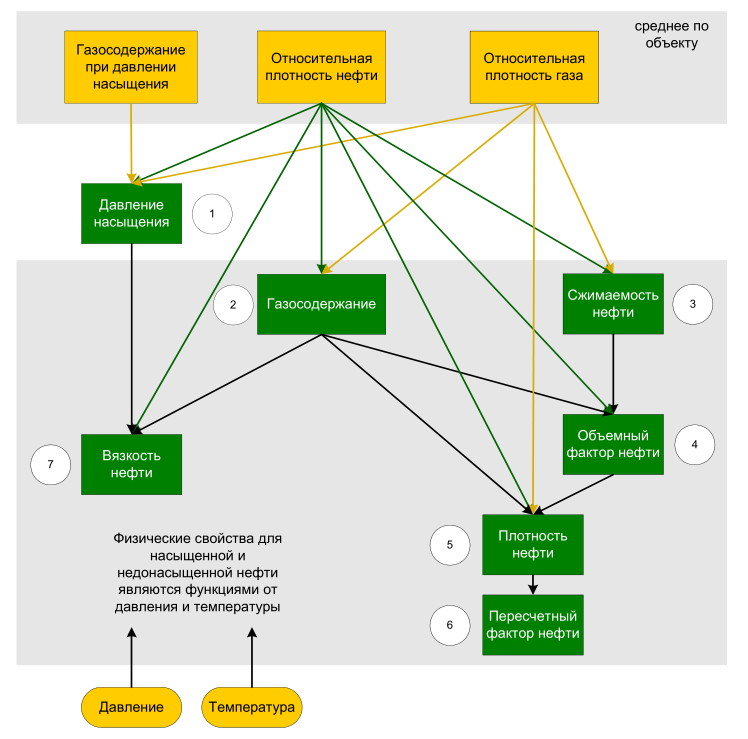
\includegraphics[width=0.8\linewidth]{PVT_props}}
	\caption{Схема взаимной связи PVT параметров нефти для модели black oil \cite{Yukos_PVT_2002}}
	\label{ris:PVT_props}
\end{figure}

В \unf{} реализована возможность проведения расчётов по нескольким наборам корреляций - набору на основе корреляций Стендинга, на основе корреляций МакКейна. PVT корреляции позволяют восстановить все необходимые для расчётов параметры из минимального набора исходных данных - плотности газа $\gamma_g$, плотности дегазированной нефти $\gamma_o$ и газосодержания при давлении насыщения $r_{sb}$. 

% хорошо бы тут привести таблицу с более подробным описание наборов корреляций 

Выбор корректного набора корреляций позволит более корректно описать поведение системы <<пласт - скважина - скважинное оборудование>>. 

На практике для повышения точности моделирования широко применяется задание расширенного набора исходных PVT параметров - калибровочных параметров: давления насыщения $P_b$, объёмного коэффициента нефти при давлении насыщения $B_{ob}$, вязкости нефти при давлении насыщения $\mu_{ob}$. 

Применение калибровочных параметров значительно снижает зависимость результатов расчётов от выбора корреляции, хотя и не устраняет такую зависимость полностью. Поэтому при отсутствии других соображений, рекомендуется использовать для расчётов набор на основе корреляций Стендинга (быстрее считает по сравнению с МакКейном) и применять калибровочные параметры.

Также полезно помнить, что калибровочные параметры, могут значительно искажать результаты рассчитанные по корреляциям. Например корреляция может дать давление насыщения $P_b$ около 100 бар. Если вы введёте калибровочное значение давления насыщения $P_b$ 20 бар, программной ошибки в расчёте не возникнет, но в реальности расхождение давления насыщения по корреляции от фактического в 5 раз маловероятно. Скорее всего, в этом случае данные не корректны. Возможность возникновения подобных рассогласований данных следует всегда иметь в виду и применять калибровочные параметры с осторожностью.  

\section{Стандартные условия} 
Многие параметры нефти, газа и воды существенно зависят от давления и температуры. Например объем занимаемый определённым количеством газа примерно в два раза снизится при повышении давления в два раза. 

Поэтому для удобства фиксации и сравнения параметров они часто приводятся к стандартным или нормальным условиям - определённым давлениям и температуре. 
	
	Принятые в разных дисциплинах и разных организациях точные значения давления и температуры в стандартных условиях могут различаться (смотри например \url{https://en.wikipedia.org/wiki/Standard_conditions_for_temperature_and_pressure}), поэтому указание значений физических величин без уточнения условий, в которых они приводятся, может приводить к ошибкам. Наряду с термином «стандартные условия» применяется термин «нормальные условия». «Нормальные условия» обычно отличаются от «стандартных» тем, что под нормальным давлением принимается давление равное 101 325 Па = 1 атм = 760 мм рт. ст.
	
	Обычно в монографиях SPE принято, что стандартное давление для газов, жидкостей и твёрдых тел, равное $10^5$ Па (100 кПа, 1 бар); стандартная температура для газов, равная 15.6 °С соответствующая 60 °F. 
	
	В Российском ГОСТ 2939-63  принято, что стандартное давление для газов, жидкостей и твёрдых тел, равное $10.13^5$ Па (101325 Па, 1 атм); стандартная температура для газов, равная 20 °С соответствующая 68 °F. 
	
	В \unf{} приняты следующие значения стандартных условий
	
	
	\begin{listing}[H]
		\begin{minted}[fontsize=\small]{vb.net}
		Public Const const_psc_atma As Double = 1
		Public Const const_tsc_C = 20
		Public Const const_convert_atma_Pa = 101325
		\end{minted}
%	\caption{Принятые параметры стандартных условий в расчетах}
%	\label{lst:code_standard_cond}
	\end{listing}

\section{Кодирование PVT свойств в строке.}
Свойства пластовых флюидов должны быть заданы для любого расчёта связанного с добычей нефти. Для полного задания свойств флюидов в модели \unf{} требуется указать более 10 параметров. Это не всегда бывает удобно делать, особенно если проводится расчёт с использованием нескольких функций. Необходимость контролировать большое количество входных параметров функций на расчётном листе Excel может приводить к ошибкам, опечаткам.

Для удобства в большинстве функций \unf{} \ создан режим упрощённого задания PVT параметров с использованием кодирования в строке. Кодирование осуществляется функциями \mintinline{vb.net}{encode_PVT_prop} и \mintinline{vb.net}{encode_PVT_stream}. Результатом кодирования является  строка в формате json, содержащая данные обо всех необходимых параметрах. Строку можно использовать в качестве аргумента в расчётах требующих указания PVT свойств.   

\putlisting{listings/PVT_encode_string.lst}

Закодировать json строку можно универсальной функцией \mintinline{vb.net}{encode_json} передав в неё ссылку на диапазон ячеек содержащих необходимые параметры и их значения. При этом должны использоваться строго заданные наименования параметров. 

Все доступные параметры флюида (по состоянию для версии 7.26) перечислены в таблице ниже

\begin{center}
	\begin{tabular}{ |m{8em}|m{15em}|m{7.5em}| } 
		\hline
		Параметр & Описание & Примечание \\ 
		\hline
		\mintinline{vb.net}{gamma_gas} & удельная плотность газа & обязательный \\ 
		\mintinline{vb.net}{gamma_oil} & удельная плотность нефти & обязательный \\ 
		\mintinline{vb.net}{gamma_wat} & удельная плотность воды & опциональный \\ 
		\mintinline{vb.net}{rsb_m3m3} & газосодержание при давлении насыщения & обязательный \\ 
		\hline
		\mintinline{vb.net}{pb_atma} & давление насыщения & калибровочный\\ 
		\mintinline{vb.net}{t_res_C} & пластовая температура & калибровочный\\ 
		\mintinline{vb.net}{bob_m3m3} & объёмный коэффициент нефти при давлении насыщения & калибровочный\\
		\mintinline{vb.net}{muob_cP} & вязкость нефти при давлении насыщения & калибровочный \\
		\hline
		\mintinline{vb.net}{PVT_corr_set} & номер набора корреляционных зависимостей & опциональный \\
		\hline
	\end{tabular}
\end{center}

Калибровочные параметры опциональны - если их не задать, соответствующие значения будут рассчитаны по корреляциям.
Все доступные параметры потока флюидов (по состоянию для версии 7.26) перечислены в таблице ниже

\begin{center}
	\begin{tabular}{  |m{11em}|m{12em}|m{7.5em}| } 
		\hline
		Параметр & Описание & Примечание \\ 
		\hline
		\mintinline{vb.net}{q_liq_sm3day} & дебит жидкости & обязательный \\ 
		\mintinline{vb.net}{fw_perc} & обводненность & обязательный \\ 
		\mintinline{vb.net}{rp_m3m3} & газовый фактор & опциональный \\ 
		\mintinline{vb.net}{q_gas_free_sm3day} & дебит свободного газа & опциональный \\ 
		\hline
	\end{tabular}
\end{center}

%Декодировать строку PVT свойств можно с использованием функции  \mintinline{vb.net}{PVT_decode_string}. Результатом работы функции декодирования является либо экземпляр класса \mintinline{vb.net}{CPVT}, который можно использовать в VBA функциях для проведения расчетов, либо PVT строка демонстрирующая корректность декодирования. 

%\putlisting{listings/PVT_decode_string.lst}

\mintinline{vb.net}{u7_Excel_functions_service} - модуль в котором можно найти функции кодирования. 

\section{Преобразования потоков флюидов}
При движения потока флюидов в системе нефтедобычи он может изменяться за счёт смешения различных потоков или разделения одного потока на несколько.

Простые преобразования потоков могут быть рассчитаны с использованием пользовательских функций \unf{} начинающихся с префикса \mintinline{vb.net}{PVT_mod_} -- PVT modification functions.
\begin{itemize}
	\item сепарация части свободного газа из потока
	\item смешение двух потоков
	\item разделение потока флюидов с произвольными параметрами
\end{itemize}

\subsection{PVT\_mod\_separate\_gas - сепарация части свободного газа из потока}

Функция \mintinline{vb.net}{feed_mod_separate_gas} описывает процесс сепарации свободного газа из потока, например на приёме УЭЦН или в газосепараторе.
После отделения части свободного газа из потока, свойства потока по прежнему могут быть описаны в рамках модели нелетучей нефти, но с несколько модифицированными параметрами, учитывающими изменение фазового состава. Функция \mintinline{vb.net}{feed_mod_separate_gas} как раз рассчитывает такие параметры.

Алгоритм модификации параметров потока сводится к снижению газового фактора и расхода свободного газа, что удаляет газ из потока. При необходимости проводится корректировка давления насыщения $P_b$, объёмного коэффициента при давлении насыщения $B_{ob}$ и вязкости при давлении насыщения $\mu_{ob}$. 

Как правило, сепарация газа из потока проводится при относительно низком давлении, например при давлении на приёме насоса. Для потока в трубах предполагается, что  в каждый момент времени все фазы потока находятся в термодинамическом равновесии, что позволяет применять корреляции для нелетучей нефти.  Однако при поступлении частично дегазированного потока в насос, давление в нем резко повышается на значительную величину (для центробежного насоса с производительностью 150 м$^3$/сут, время прохождения потоком через одну ступень составляет около 0.02 сек \cite{diss_Igrevesky_ESP_gas}, таким образом через ЭЦН с 400 ступеней поток будет двигаться порядка 10 сек. При этом давление может повыситься на величину порядка 200 атм). За такое время свободный газ оставшийся в потоке может не успеть достичь термодинамического равновесия с нефтью, или другими слова может не успеть полностью раствориться. В работе Игревского В.И. \cite{diss_Igrevesky_ESP_gas} для учёта этого эффекта вводится коэффициент фазной неравновесности $K_f$

$$K_f = \frac{V_{sol}}{V_{eq}}= \frac{Q_{g.sol}}{Q_{g.eq}}$$

где  $V_{sol}$ - объем газа который растворится в нефти при движении через ЭЦН, $V_{sol}$ - объем газа который растворился бы в нефти при движении через ЭЦН при достижении термодинамического равновесия. 

Величина $K_f$ зависит среди прочих параметров от дисперсности потока (размера пузырьков газа), и объёмного газосодержания.  Для грубодисперсных смесей газ - вода можно принять $K_f=0.2$, для тонкодисперсных от $K_f=0.7$ до $K_f=1$. Для газонефтяных смесей можно считать $K_f=1$, то есть весь газ успевает раствориться в нефти при движении через ЭЦН. Это же предположении может быть использовано при движении газонефтяной смеси через трубы (скорость движения меньше в 5 - 10 раз в НКТ по сравнению с ЭЦН).

Для оценки влияния фазной неравновесности нефти на параметры многофазного потока при сепарации газа из потока можно использовать параметр \mintinline{vb.net}{gas_goes_into_solution}, который определяет значение   $K_f$

При условии $K_f = 0$ -- газ выделившийся в свободное состояние не растворяется обратно в нефти, при $K_f = 1$ -- весь газ может раствориться при повышении давления.

Новый газовый фактор и расход свободного газа, после сепарации газа можно найти из условия
\begin{equation}
	r_p^{new} = r_p - \left( r_p - r_s \right) k_{sep} 
\end{equation}

\begin{equation}
q_{gas}^{new} = q_{gas}(1-k_{sep}) 
\end{equation}

Максимально возможное значение газосодержания при повышении давления можно найти из выражения

\begin{equation} 
	r_s^{max} = r_s + \left( r_p - r_s \right) (1 - k_{sep}) *K_f 
	\label{eq:rsmax}
\end{equation}

При повышении давления часть газа может раствориться в нефти, что можно описать найдя величины $P_{b}^{new}$, $B_{ob}^{new}$,$\mu_{ob}^{new}$ c учетом максимально достижимого значения газосодержания (\ref{eq:rsmax}).

$$P_{b}^{new} = P_b(r_s^{max}) $$

$$B_{ob}^{new} = B_{ob}(r_s^{max}) $$

$$\mu_{ob}^{new} = \mu_{ob}(r_s^{max}) $$

где соответствующие зависимости $P_{b}(r_s)$, $B_{o}(r_s)$,$\mu_{o}(r_s)$ определяются в соответствии с заданным набором корреляций.

Рассмотрим пример 1 преобразования свойств потока флюида для следующего набора параметров:
параметры сепарации:  $k_{sep} = 0.5$ ,$p_{sep} = 50$   атма,	$t_{sep} = 90$   C ,$K_f = 0 $.    


\begin{table}[ht]
	\centering
	\caption{Исходные данные и результаты расчёта модификации флюида после частичной сепарации свободного газа. Пример 1, $K_f=0$ -- газ не растворяется при повышении давления.}
	\begin{tabular}{ |c|c|c|} 
		\hline
		Параметр & Исходные значения & Модифицированные \\ 
		\hline
		$\gamma_g$ 				&$0.9$	& $0.9$    \\ 
		$\gamma_o$ 					&$0.9$	& $0.9$   \\ 
		$r_{sb}$ ,  м$^3$/м$^3$ 		&$80$	& $25$ \\ 
		$P_b$ , атма 					&$130$	& $50$ 	 \\ 
		$T_{res} $,  C 					&$90$	& $90$ \\ 
		$B_{ob} $ , м$^3$/м$^3$  		&$1.2$	& $1.09$ \\ 
		$\mu_{ob}  $,  сП  				&$1$	& $1.96$   \\ 
		\hline
		$Q_{gas\ free}  $,  м$^3$/сут  	&$1000$	& $500$  \\ 
		$Q_{liq}  $,  м$^3$/сут  			&$15$	& $15$ \\ 
		$f_{w}  $,  \%  					&$1$	& $1$  \\ 
		$r_p  $,  м$^3$/м$^3$  			&$80$	& $52$ \\ 
		\hline
	\end{tabular}
	\label{table:separ_gas_table_1}
\end{table}

Зависимости свойств флюида от давления для примера 1 приведены на рисунке \ref{ris:separ_gas_plot_1}.

\begin{figure}[ht]
\begin{tikzpicture}[scale=0.65]
	\begin{axis}[
		xlabel=$P \;  atma$,
		ylabel=$r_s\; m^3/m^3$,
		legend pos=north west,
		title=газосодержание]
		\addplot table [y=rs, x=P]{data/separ_gas.txt};
		\addlegendentry{original}
		\addplot table [y=rs_mod, x=P]{data/separ_gas.txt};
		\addlegendentry{modified}
	\end{axis}
\end{tikzpicture}
\begin{tikzpicture}[scale=0.65]
	\begin{axis}[
		xlabel=$P \;  atma$,
		ylabel=$B_o\; m^3/m^3$,
		legend pos=north west,
		title=объемный коэффициент нефти]
		\addplot table [y=bo, x=P]{data/separ_gas.txt};
		\addlegendentry{original}
		\addplot table [y=bo_mod, x=P]{data/separ_gas.txt};
		\addlegendentry{modified}
	\end{axis}
\end{tikzpicture}
\begin{tikzpicture}[scale=0.65]
	\begin{axis}[
		xlabel=$P \;  atma$,
		ylabel=$\mu_o\; cP$,
		legend pos=north east,
		title=вязкость нефти]
		\addplot table [y=muo, x=P]{data/separ_gas.txt};
		\addlegendentry{original}
		\addplot table [y=muo_mod, x=P]{data/separ_gas.txt};
		\addlegendentry{modified}
	\end{axis}
\end{tikzpicture}
\caption{Зависимость параметров флюида от давления до и после сепарации части свободного газа. Пример 1, $K_f=0$ -- газ не растворяется при повышении давления}
\label{ris:separ_gas_plot_1}
\end{figure}

Из приведённых рисунков видно, что свойства нефти при давлении ниже давления сепарации не изменились, а новое давление насыщения показывает, что при повышении давления газ не будет растворяться в нефти. При этом значения параметров потока жидкости $Q_{liq}, f_w$ не изменяются.

При увеличении коэффициента неравновесности $K_f=0.9$ картина изменится - эффективное значение давления насыщения нефти вырастет, что позволит части газа раствориться. Ниже приводится пример 2, где также для наглядности изменён набор корреляций для следующего набора параметров: $k_{sep} = 0.5$ ,$p_{sep} = 50$   атма,	$t_{sep} = 90$   C ,$K_f = 0.9 $. Результаты расчета приведены в таблице \ref{table:separ_gas_table_2} и на   рисунке \ref{ris:separ_gas_plot_2}.

Следует отметить, что на величину эффективного значения давления насыщения может значительно влиять выбор набора корреляций для расчёта PVT свойств, в частности корреляции для зависимости давления насыщения от газосодержания при давлении насыщения. 

\begin{table}[H]
	\centering
	\caption{Исходные данные и результаты расчёта модификации флюида после частичной сепарации свободного газа. Пример 2, $K_f=0.9$ -- газ частично растворяется при повышении давления.}
	\begin{tabular}{ |c|c|c|} 
		\hline
		Параметр & Исходные значения & Модифицированные \\ 
		\hline
		$\gamma_g$ 				&$0.9$	& $0.9$    \\ 
		$\gamma_o$ 					&$0.9$	& $0.9$   \\ 
		$r_{sb}$ ,  м$^3$/м$^3$ 		&$80$	& $61$ \\ 
		$P_b$ , атма 					&$130$	& $84$ 	 \\ 
		$T_{res} $,  C 					&$90$	& $90$ \\ 
		$B_{ob} $ , м$^3$/м$^3$  		&$1.2$	& $1.16$ \\ 
		$\mu_{ob}  $,  сП  				&$1$	& $1.22$   \\ 
		\hline
		$Q_{gas\ free}  $,  м$^3$/сут  	&$1000$	& $500$  \\ 
		$Q_{liq}  $,  м$^3$/сут  			&$15$	& $15$ \\ 
		$f_{w}  $,  \%  					&$1$	& $1$  \\ 
		$r_p  $,  м$^3$/м$^3$  			&$80$	& $63$ \\ 
		\hline
	\end{tabular}
\label{table:separ_gas_table_2}
\end{table}

Зависимости свойств флюида от давления для примера 2 приведены на рисунке \ref{ris:separ_gas_plot_2}.

\begin{figure}[H]
\begin{tikzpicture}[scale=0.65]
	\begin{axis}[
		xlabel=$P \;  atma$,
		ylabel=$r_s\; m^3/m^3$,
		legend pos=north west,
		title=газосодержание]
		\addplot table [y=rs, x=P]{data/separ_gas_1.txt};
		\addlegendentry{original}
		\addplot table [y=rs_mod, x=P]{data/separ_gas_1.txt};
		\addlegendentry{modified}
	\end{axis}
\end{tikzpicture}
\begin{tikzpicture}[scale=0.65]
	\begin{axis}[
		xlabel=$P \;  atma$,
		ylabel=$B_o\; m^3/m^3$,
		legend pos=north west,
		title=объемный коэффициент нефти]
		\addplot table [y=bo, x=P]{data/separ_gas_1.txt};
		\addlegendentry{original}
		\addplot table [y=bo_mod, x=P]{data/separ_gas_1.txt};
		\addlegendentry{modified}
	\end{axis}
\end{tikzpicture}
\begin{tikzpicture}[scale=0.65]
	\begin{axis}[
		xlabel=$P \;  atma$,
		ylabel=$\mu_o\; cP$,
		legend pos=north east,
		title=вязкость нефти]
		\addplot table [y=muo, x=P]{data/separ_gas_1.txt};
		\addlegendentry{original}
		\addplot table [y=muo_mod, x=P]{data/separ_gas_1.txt};
		\addlegendentry{modified}
	\end{axis}
\end{tikzpicture}
\caption{Зависимость параметров флюида от давления до и после сепарации части свободного газа. Пример 2, $K_f=0.9$ -- газ частично растворяется при повышении давления}
\label{ris:separ_gas_plot_2}
\end{figure}


Часть настроек управляющая выводом результатов задается в виде закодированной строки в аргументе \mintinline{vb.net}{param}.

\begin{table}[H]
	\caption{Параметры функции \mintinline{vb.net}{feed_mod_separate_gas} передаваемые через аргумент -- \mintinline{vb.net}{param}}
	\label{table:param_list_feed_med_separation}
	\begin{tabular}{p{0.4\textwidth}p{0.55\textwidth}}
		\hline
		Ключ & Описание  \\ \hline
		\mintinline{vb.net}{show_array} & Показывать расширенные результаты расчета: 0 -- результат в виде одного числа (значение по умолчанию), 1 -- результат в виде массива.    \\ \hline
		
		\mintinline{vb.net}{show_log} & Показывать лог расчета в выводе. 0 -- лог выводиться не будет, 1 -- будет показан лог в виде json строки в массиве вывода. Большой размер лога может вызвать проблемы на некоторых версиях Excel.   \\ \hline
		
		\mintinline{vb.net}{gas_goes_into_solution} & Коэффициент фазной неравновесности $K_f$  \\ \hline
		
	\end{tabular}
\end{table}

При включенной опции \mintinline{vb.net}{show_array=1} результат выдается в виде двумерного массива значений - плоской таблицы. Результирующая таблица может быть непосредственно выведена в ячейки Excel (в версиях не поддерживающие динамические массивы необходимо использовать Cntrl-Shift-Enter для вывода результата в заранее выделенный диапазон ячеек) или получена в виде массива при вызове из VBA.

При выводе массива на лист Excel первая строка содержит значения параметров, вторая подписи к значениям. При выводе с использованием Cntrl-Shift-Enter можно вывести только первую строку параметров и распространить расчетную формулу протягиванием на несколько строк.

\begin{table}[H]
	\caption{Расширенный вывод функции \mintinline{vb.net}{feed_mod_separate_gas}}
	\label{table:param_list}
	\begin{tabular}{p{0.05\textwidth}p{0.3\textwidth}p{0.545\textwidth}}
		\hline
		№& Параметр & Описание  \\ \hline
		0 & \mintinline{vb.net}{feed} & json строка описывающая параметры модифицированного потока флюидов    \\ \hline
		
		1 & \mintinline{vb.net}{log} & Лог расчета, выводится при \mintinline{vb.net}{show_log = 1}  \\ \hline
		
	\end{tabular}
\end{table}
 

\section{Соотношение некоторых свойств пластовых флюидов}
Приведем в этом разделе несколько картинок, рассчитанных с использованием \unf{} показывающих соотношение некоторых параметров для различных типов флюидов. Расчет проведен с использованием \mintinline{vb.net}{ex010.PVT.xlsm} и его можно повторить.
Картинки представляются интересными и полезными, но не вписываются в описание отдельных функций, поэтому приводятся тут.
Интересное наблюдение по этим графикам - это то, что свойства газа сильно отличаются от свойств жидкости. При этом свойства газа сильно меняются с давлением. 

\begin{figure}[H]
	\center{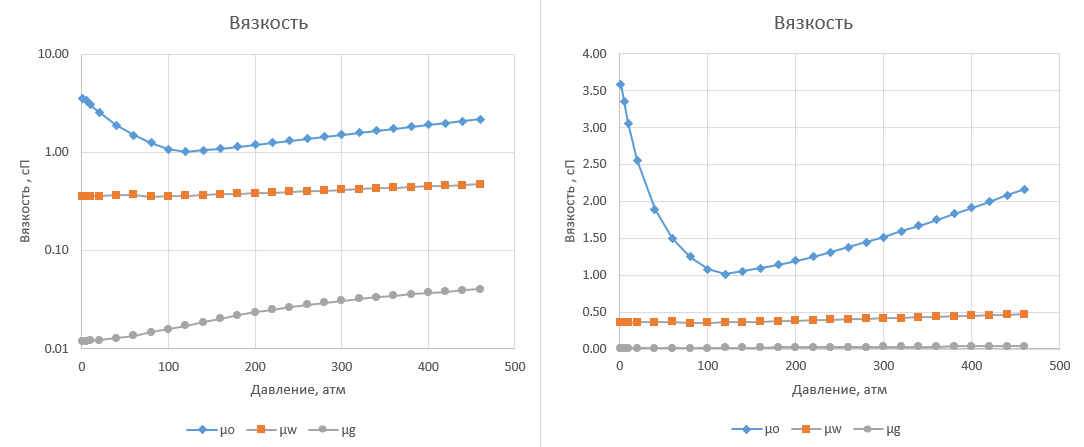
\includegraphics[width=1\linewidth]{viscosity_plot}}
	\caption{Зависимость вязкости от давления для нефти, газа и воды. Обычные и полулогарифмические координаты}
	\label{ris:viscosity_plot}
\end{figure}

Вязкость газа сильно меньше чем для нефти и воды, поэтому ее логично показать в полулогарифмических координатах. Также заметно для нефти, что давление насыщения сильно влияет.

\begin{figure}[H]
	\center{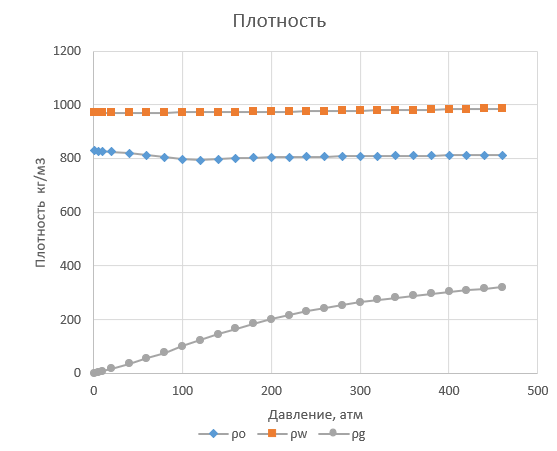
\includegraphics[width=0.6\linewidth]{density_plot}}
	\caption{Зависимость плотности от давления для нефти, газа и воды}
	\label{ris:density_plot}
\end{figure}

Плотность газа сильно растет с давлением, но при этом в диапазоне интереса остается заметно ниже плотности нефти и воды.

\begin{figure}[H]
	\center{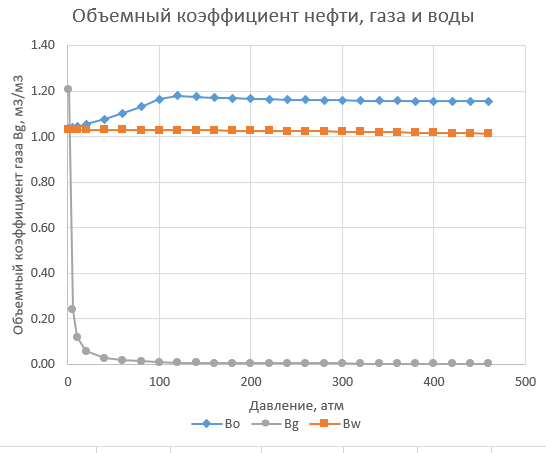
\includegraphics[width=0.6\linewidth]{FVF_plot}}
	\caption{Зависимость объемного коэффициента от давления для нефти, газа и воды}
	\label{ris:FVF_plot}
\end{figure}

\begin{figure}[H]
	\center{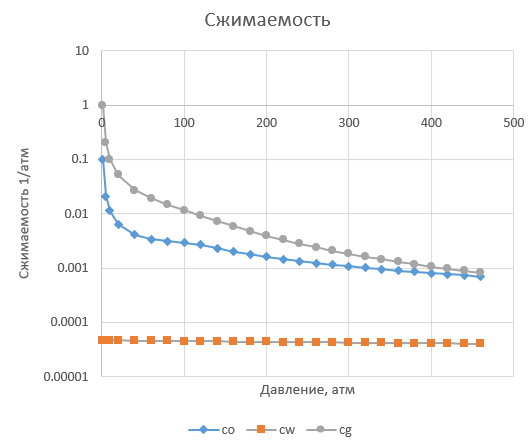
\includegraphics[width=0.6\linewidth]{compressibility_plot}}
	\caption{Зависимость сжимаемости от давления для нефти, газа и воды}
	\label{ris:compressibility_plot}
\end{figure}

Объемный коэффициент и сжимаемость непосредственно связаны между собой. Для нефти это справедливо только для насыщенной нефти. 
$$ B=B_{ref} e^{c(p-p_{ref})}$$

Для газа сжимаемость зависит от z фактора
$$c_g = \frac{1}{p} - \frac{1}{z} \frac{dz}{dp}$$

\begin{figure}[H]
	\center{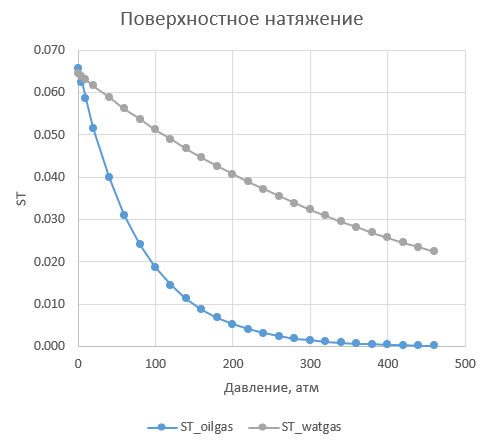
\includegraphics[width=0.6\linewidth]{st_plot}}
	\caption{Зависимость коэффициента поверхностного натяжения нефть-газ и вода-газ от давления}
	\label{ris:st_plot}
\end{figure}

\begin{figure}[H]
	\center{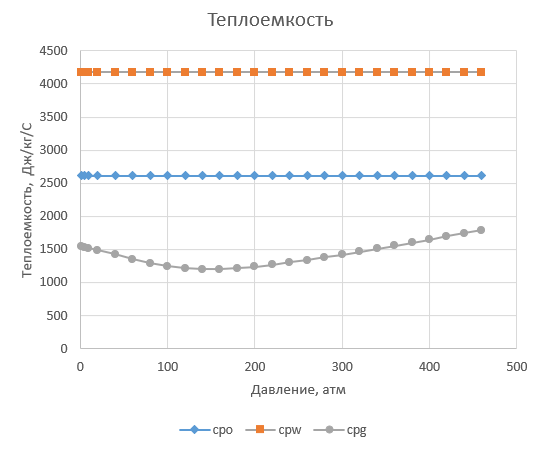
\includegraphics[width=0.6\linewidth]{heat_cap_plot}}
	\caption{Зависимость теплоемкости при постоянном давлении от давления}
	\label{ris:heat_cap_plot}
\end{figure}

\subsection{PVT\_pb\_atma давление насыщения}
Функция рассчитывает давление насыщения по известным данным газосодержания при давлении насыщения, $\gamma_g, \gamma_o, T_r$.

При проведении расчётов с использованием значения давления насыщения, следует помнить, что давление насыщения является функцией температуры. В частности при калибровки результатов расчётов на известное значение давления насыщения $P_b$ следует указывать значение пластовой температуры $T_r$ при котором давление насыщения было получено. 

В наборе корреляций на основе корреляции Стендинга расчет давления насыщения проводится по корреляции Стендинга \cite{Yukos_PVT_2002}

\putlisting{listings/PVT_Pb_atma.lst}

Пример расчёта с использованием функции \mintinline{vb.net}{PVT_pb_atma} для различных наборов PVT корреляций приведён на рисунке ниже. Видно, что результаты расчетов по различным корреляциях дают качественно схожие результаты, но не совпадают друг с другом.  Отличия, по всей видимости,  обусловленные применением различных наборов исходных данных, использовавшихся авторами. Поэтому при проведении расчетов для конкретного месторождения актуальной является задача выбора адекватного набора корреляций. Макросы \unf{} позволяют провести расчет с использованием различных подходов, но при этом выбор корреляции остается за пользователем. 

\begin{tikzpicture}[scale=0.8]
\begin{axis}[
xlabel=$r_{sb} \;  m^3/m^3$,
ylabel=$P_b\; atma$,
legend pos=north west,
title=Standing]
\addplot table [y=T20, x=Rs]{data/Pb_T_data.txt};
\addlegendentry{$T = 20$ °С}
\addplot table [y=T60, x=Rs]{data/Pb_T_data.txt};
\addlegendentry{$T = 60$ °С}
\addplot table [y=T100, x=Rs]{data/Pb_T_data.txt};
\addlegendentry{$T = 100$ °С}
\addplot table [y=T140, x=Rs]{data/Pb_T_data.txt};
\addlegendentry{$T = 140$ °С}
\end{axis}
\end{tikzpicture}
\begin{tikzpicture}[scale=0.8]
\begin{axis}[
xlabel=$r_{sb} \;  m^3/m^3$,
ylabel=$P_b\; atma$,
legend pos=north west,
title = McCain]
\addplot table [y=T20, x=Rs]{data/Pb_T_data1.txt};
\addlegendentry{$T = 20$ °С}
\addplot table [y=T60, x=Rs]{data/Pb_T_data1.txt};
\addlegendentry{$T = 60$ °С}
\addplot table [y=T100, x=Rs]{data/Pb_T_data1.txt};
\addlegendentry{$T = 100$ °С}
\addplot table [y=T140, x=Rs]{data/Pb_T_data1.txt};
\addlegendentry{$T = 140$ °С}
\end{axis}
\end{tikzpicture}


При проведении расчётов с использованием набора корреляций на основе корреляций МакКейна следует учитывать, что они работают только для температур более 18 $^\circ$C. При более низких значениях температуры расчёт будет проводиться для 18 $^\circ$C.

Обратите внимание, что для функции \mintinline{vb.net}{PVT_pb_atma} набор аргументов отличается от набора для всех остальных функций PVT. Для расчёта давления насыщения нет необходимости задавать давление при котором будет проведён расчёт, так как давление является результатом расчёта.

\subsection{PVT\_rs\_m3m3 – газосодержание}

Газосодержание это отношения объёма газа растворённого в нефти приведённого к стандартным условиям к объёму дегазированной нефти приведённой к стандартным условиям. 

$$r_s = \frac{V_{g,sc}}{V_{o,sc}}$$

Газосодержание является одним из ключевых свойств нефти при расчётах производительности скважин и работы скважинного оборудования. Динамика изменения газосодержания при изменении давления и температуры во многом определяет количество свободного газа в потоке и должна учитываться при проведении расчётов. 

При задании PVT свойств нефти часто используют значение газосодержания при давлении насыщения $r_{sb}$ - определяющее объем газа растворенного в нефти в пластовых условиях. В модели флюида \unf{} газосодержание при давлении насыщения является исходным параметром нефти и должно быть обязательно задано. 

Следует отличать газосодержание в нефти при давлении насыщения $r_{sb}$ и газовый фактор $r_p$.

$$r_p = \frac{Q_{g,sc}}{Q_{o,sc}}$$

Газовый фактор $r_{p}$  в отличии от газосодержания $r_{sb}$  является, вообще говоря, параметром скважины - показывает отношение объёма добытого из скважины газа  к объёму добытой нефти приведённые к стандартным условиям. Газосодержание же является свойством нефти - показывает сколько газа растворено в нефти. Если газ добываемый из скважины это газ который выделился из нефти в процессе подъёма, что характерно для недонасыщенных нефтей, то значения газового фактора и газосодержания будут совпадать. Если газ поступает в скважину не непосредственно из добываемой нефти, а например фильтруется из газовой шапки или поступает через негерметичность ствола скважины - то в такой скважине газовый фактор может значительно превышать значение газосодержания. Такая ситуация может быть смоделирована в \unf{}. Для этого необходимо наряду с газосодержанием при давлении насыщения $r_{sb}$ задать значение газового фактора $r_p$. В этом случае газосодержание при давлении насыщения $r_{sb}$  будет определять динамику выделения попутного газа из нефти при снижении давления, а газовый фактор $R_p$ определять общее количество газа в потоке. 

При определённых условиях газовый фактор может быть меньше газосодержания. Это происходит, когда газ выделяется в призабойной зоне и скапливается в ней, не поступая в скважину вместе с нефтью. При этом в скважину поступает частично дегазированная нефть. Такие условия возникают редко, требуют определённого набора параметров, существуют на скважине ограниченное время и представляют интерес больше для разработчиков нежели чем для технологов. С точки зрения анализа работы скважины и скважинного оборудования можно считать, что значение газового фактора не может быть меньше газосодержания при давлении насыщения. Такой предположение реализовано в \unf{}. При этом значение газового фактора технически легче измерить чем газосодержание - поэтому при противоречии значений газового фактора и газосодержания при давлении насыщения приоритет отдается газовому фактору. 

\putlisting{listings/PVT_Rs_m3m3.lst}

Примеры расчёта с использованием функции \mintinline{vb.net}{PVT_Rs_m3m3} для различных наборов PVT корреляций приведён на рисунке ниже.

\newcommand{\RsDataFile}{data/Rs_P_data.txt}
\begin{tikzpicture}[scale=0.8]
\begin{axis}[
xlabel=$r_{sb} \;  m^3/m^3$,
ylabel=$P_b\; atma$,
legend pos=south east,
title=Standing]
\addplot table [y=T_0_20, x=P]{\RsDataFile};
\addlegendentry{$T = 20$ °С}
\addplot table [y=T_0_60, x=P]{\RsDataFile};
\addlegendentry{$T = 60$ °С}
\addplot table [y=T_0_100, x=P]{\RsDataFile};
\addlegendentry{$T = 100$ °С}
\addplot table [y=T_0_140, x=P]{\RsDataFile};
\addlegendentry{$T = 140$ °С}
\end{axis}
\end{tikzpicture}
\begin{tikzpicture}[scale=0.8]
\begin{axis}[
xlabel=$r_{sb} \;  m^3/m^3$,
ylabel=$P_b\; atma$,
legend pos=south east,
title = McCain]
\addplot table [y=T_1_20, x=P]{\RsDataFile};
\addlegendentry{$T = 20$ °С}
\addplot table [y=T_1_60, x=P]{\RsDataFile};
\addlegendentry{$T = 60$ °С}
\addplot table [y=T_1_100, x=P]{\RsDataFile};
\addlegendentry{$T = 100$ °С}
\addplot table [y=T_1_140, x=P]{\RsDataFile};
\addlegendentry{$T = 140$ °С}
\end{axis}
\end{tikzpicture}


\subsection{PVT\_bo\_m3m3 – объёмный коэффициент нефти}

Функция рассчитывает объёмный коэффициент нефти для произвольных термобарических условий. 
Объёмный коэффициент нефти определяется как отношение объёма занимаемого нефтью в пластовых условиях к объёму занимаемому нефтью при стандартных условиях. 

$$B_o = \frac{V_{o,rc}}{V_{o,sc}}$$

Нефть в пласте занимает больший объем, чем на поверхности, за счёт растворенного в ней газа. Соответственно объёмный коэффициент нефти обычно имеет значение больше единицы при давлениях больше чем стандартное.

Для калибровки значения объёмного коэффициента можно использовать значение объёмного коэффициента нефти при давлении насыщения $B_{ob}$. 

Следует отметить, что вообще говоря значение объёмного коэффициента нефти при давлении насыщения не является значением при пластовых условиях (при давлении выше давления насыщения играет роль сжимаемость нефти), однако при анализе производительности скважины и скважинного оборудования можно условно считать, что значение объёмного коэффициента при давлении насыщения соответствует значению  объёмного коэффициента в пластовых условиях.  

\putlisting{listings/PVT_Bo_m3m3.lst}

Примеры расчёта с использованием функции \mintinline{vb.net}{PVT_bo_m3m3} для различных наборов PVT корреляций приведены на рисунках ниже.

Объёмный коэффициент нефти хорошо коррелирует со значением газосодержания. Поэтому различный вид кривых на рисунке ниже связан с первую очередь с различным газосодержанием при проведении расчётов.

\newcommand{\BoDataFile}{data/Bo_P_data.txt}
\begin{tikzpicture}[scale=0.8]
\begin{axis}[
xlabel=$P\; atma$,
ylabel=$B_o\;  m^3/m^3$,
legend pos=south east,
title=Standing]
\addplot table [y=T_0_20, x=P]{\BoDataFile};
\addlegendentry{$T = 20$ °С}
\addplot table [y=T_0_60, x=P]{\BoDataFile};
\addlegendentry{$T = 60$ °С}
\addplot table [y=T_0_100, x=P]{\BoDataFile};
\addlegendentry{$T = 100$ °С}
\addplot table [y=T_0_140, x=P]{\BoDataFile};
\addlegendentry{$T = 140$ °С}
\end{axis}
\end{tikzpicture}
\begin{tikzpicture}[scale=0.8]
\begin{axis}[
xlabel=$P\; atma$,
ylabel=$B_o\;  m^3/m^3$,
legend pos=south east,
title = McCain]
\addplot table [y=T_1_20, x=P]{\BoDataFile};
\addlegendentry{$T = 20$ °С}
\addplot table [y=T_1_60, x=P]{\BoDataFile};
\addlegendentry{$T = 60$ °С}
\addplot table [y=T_1_100, x=P]{\BoDataFile};
\addlegendentry{$T = 100$ °С}
\addplot table [y=T_1_140, x=P]{\BoDataFile};
\addlegendentry{$T = 140$ °С}
\end{axis}
\end{tikzpicture}

\subsection{PVT\_bg\_m3m3 – объёмный коэффициент газа}
Функция рассчитывает объёмный коэффициент нефтяного газа для произвольных термобарических условий. 

Объёмный коэффициент газа определяется как отношение объёма, занимаемого газом для произвольных термобарических условий (при определённом давлении и температуре), к объёму, занимаемому газом при стандартных условиях. 

$$B_g = \frac{V_{g,rc}(P,T)}{V_{g,sc}}$$

Значение объёмного коэффициента газа может быть определено исходя из уравнения состояния газа

$$ PV = z \nu RT  $$

откуда можно получить 

$$ B_g = z \frac{P_{sc}}{P} \frac{T}{T_{sc}} $$

где $P_{sc}, T_{sc}$ давление (атм) и температура (К) при стандартных условиях, $P,T$ давление (атм) и температура (°K) при расчетных условиях, $z$ коэффициент сверхсжимаемости газа, который вообще говоря зависит от давления и температуры $z = z(P,T)$. 

\putlisting{listings/PVT_Bg_m3m3.lst}

\newcommand{\DataFile}{data/Bg_P_data.txt}
\begin{tikzpicture}[scale=0.8]
\begin{axis}[
ymode=log, 
xlabel=$P\; atma$,
ylabel=$B_g\\;  m^3/m^3$,
legend pos=north east,
title=Standing]
\addplot table [y=T_0_20, x=P]{\DataFile};
\addlegendentry{$T = 20$ °С}
\addplot table [y=T_0_60, x=P]{\DataFile};
\addlegendentry{$T = 60$ °С}
\addplot table [y=T_0_100, x=P]{\DataFile};
\addlegendentry{$T = 100$ °С}
\addplot table [y=T_0_140, x=P]{\DataFile};
\addlegendentry{$T = 140$ °С}
\end{axis}
\end{tikzpicture}
\begin{tikzpicture}[scale=0.8]
\begin{axis}[
ymode=log, 
xlabel=$P\; atma$,
ylabel=$B_g\;  m^3/m^3$,
legend pos=north east,
title = McCain]
\addplot table [y=T_1_20, x=P]{\DataFile};
\addlegendentry{$T = 20$ °С}
\addplot table [y=T_1_60, x=P]{\DataFile};
\addlegendentry{$T = 60$ °С}
\addplot table [y=T_1_100, x=P]{\DataFile};
\addlegendentry{$T = 100$ °С}
\addplot table [y=T_1_140, x=P]{\DataFile};
\addlegendentry{$T = 140$ °С}
\end{axis}
\end{tikzpicture}

\subsection{PVT\_bw\_m3m3 – объёмный коэффициент воды}
Функция рассчитывает объёмный коэффициент воды для произвольных термобарических условий. 

Объёмный коэффициент воды определяется как отношение объёма занимаемого водой для произвольных термобарических условий (при определённом давлении и температуре) к объёму, занимаемому водой при стандартных условиях. 

$$B_w = \frac{V_{w,rc}(P,T)}{V_{w,sc}}$$

\putlisting{listings/PVT_Bw_m3m3.lst}

\subsection{PVT\_mu\_oil\_cP – вязкость нефти}
Функция рассчитывает вязкость нефти при заданных термобарических условиях по корреляции. Расчёт может быть откалиброван на известное значение вязкости нефти при давлении равном давлению насыщения и при пластовой температуре за счёт задания калибровочного параметра \mintinline{vb.net}{muob_cP}. При калибровке динамика изменения будет соответствовать расчету по корреляции, но значения будут масштабированы таким образом, чтобы при давлении насыщения удовлетворить калибровочному параметру.

При расчёте следует обратить внимание, что значение вязкости коррелирует со значением плотности нефти. Как правило вязкость тяжёлых нефтей выше чем для легких.

При расчёте с использованием набора корреляций на основе корреляции Стендинга - вязкость как дегазированной нефти и нефти с учетом растворенного газа рассчитывается по корреляции Беггса Робинсона \cite{Yukos_PVT_2002}. 
Корреляции для расчета вязкости разгазированной и газонасыщенной нефти, разработанные Beggs \& Robinson, основаны на 2000 замерах 600 различных нефтей.
Диапазоны значений основных свойств, использованных для разработки данной корреляции, приведены в таблице ниже.
\begin{center}
	\begin{tabular}{ccc}
		давление, atma & \textbf{8.96…483.} \\
		температура, °C & \textbf{37…127}  \\
		газосодержание, $r_s \; m^3 /m^3$ & \textbf{3.6…254}\\
		относительная плотность нефти по воде,, $\gamma_o$ & \textbf{0.725…0.956} \\
	\end{tabular}
\end{center}
   
\putlisting{listings/PVT_mu_oil_cP.lst}

\newcommand{\MuDataFile}{data/Muo_P_data.txt}
\begin{tikzpicture}[scale=0.8]
\begin{axis}[
xlabel=$P\; atma$,
ylabel=$\mu_o\; cP$,
legend pos=north east,
title=Standing]
\addplot table [y=T_0_20, x=P]{\MuDataFile};
\addlegendentry{$T = 20$ °С}
\addplot table [y=T_0_60, x=P]{\MuDataFile};
\addlegendentry{$T = 60$ °С}
\addplot table [y=T_0_100, x=P]{\MuDataFile};
\addlegendentry{$T = 100$ °С}
\addplot table [y=T_0_140, x=P]{\MuDataFile};
\addlegendentry{$T = 140$ °С}
\end{axis}
\end{tikzpicture}
\begin{tikzpicture}[scale=0.8]
\begin{axis}[
xlabel=$P\; atma$,
ylabel=$\mu_o\; cP$,
legend pos=north east,
title = McCain]
\addplot table [y=T_1_20, x=P]{\MuDataFile};
\addlegendentry{$T = 20$ °С}
\addplot table [y=T_1_60, x=P]{\MuDataFile};
\addlegendentry{$T = 60$ °С}
\addplot table [y=T_1_100, x=P]{\MuDataFile};
\addlegendentry{$T = 100$ °С}
\addplot table [y=T_1_140, x=P]{\MuDataFile};
\addlegendentry{$T = 140$ °С}
\end{axis}
\end{tikzpicture}

\subsection{PVT\_mu\_gas\_cP – вязкость газа}

Функция рассчитывает вязкость газа при заданных термобарических условиях. Результат расчета в сП.  Используется подход предложенный Lee  \cite{Lee_1966}, который хорошо подходит для большинства натуральных газов. 
В отличии от нефти и других жидкостей вязкость газа, как правило, значительно ниже, что определяет высокую подвижность газа. 
Более подробное описание методов расчета вязкости газа можно найти на странице  \href{http://petrowiki.org/Gas_viscosity}{http://petrowiki.org/gas\_viscosity}


\putlisting{listings/PVT_mu_gas_cP.lst}

\newcommand{\MugDataFile}{data/Mug_P_data.txt}
\begin{tikzpicture}[scale=0.8]
\begin{axis}[
xlabel=$P\; atma$,
ylabel=$\mu_g\; cP$,
legend pos=north west,
title=Standing]
\addplot table [y=T_0_20, x=P]{\MugDataFile};
\addlegendentry{$T = 20$ С}
\addplot table [y=T_0_60, x=P]{\MugDataFile};
\addlegendentry{$T = 60$ С}
\addplot table [y=T_0_100, x=P]{\MugDataFile};
\addlegendentry{$T = 100$ С}
\addplot table [y=T_0_140, x=P]{\MugDataFile};
\addlegendentry{$T = 140$ С}
\end{axis}
\end{tikzpicture}
\begin{tikzpicture}[scale=0.8]
\begin{axis}[
xlabel=$P\; atma$,
ylabel=$\mu_g\; cP$,
legend pos=north west,
title = McCain]
\addplot table [y=T_1_20, x=P]{\MugDataFile};
\addlegendentry{$T = 20$ С}
\addplot table [y=T_1_60, x=P]{\MugDataFile};
\addlegendentry{$T = 60$ С}
\addplot table [y=T_1_100, x=P]{\MugDataFile};
\addlegendentry{$T = 100$ С}
\addplot table [y=T_1_140, x=P]{\MugDataFile};
\addlegendentry{$T = 140$ С}
\end{axis}
\end{tikzpicture}

\subsection{PVT\_mu\_wat\_cP – вязкость воды}

Функция рассчитывает вязкость воды при заданных термобарических условиях. Результат расчета выдается в сП. 
Вязкость воды зависит от давления, температуры и наличия растворенных примесей. В общем вязкость воды растет при росте давления, снижении температуры, повышении солености. 
Растворение газа почти не влияет на вязкость воды и в расчетах не учитывается. 
Расчет проводится по корреляции McCain \cite{McCain_1991}

Более подробное описание методов расчета вязкости газа можно найти на странице  \href{http://petrowiki.org/Produced_water_properties}{http://petrowiki.org/Produced\_water\_properties}


\putlisting{listings/PVT_mu_wat_cP.lst}


Следует отметить, что вязкость воды достаточно сильно зависит от температуры, в то время как зависимость от давления менее выражена.

\newcommand{\MuwDataFile}{data/Muw_P_data.txt}
\begin{tikzpicture}[scale=0.8]
\begin{axis}[
xlabel=$P\; atma$,
ylabel=$\mu_w\; cP$,
legend pos=north west,
title=Standing]
\addplot table [y=T_0_20, x=P]{\MuwDataFile};
\addlegendentry{$T = 20$ °С}
\addplot table [y=T_0_60, x=P]{\MuwDataFile};
\addlegendentry{$T = 60$ °С}
\addplot table [y=T_0_100, x=P]{\MuwDataFile};
\addlegendentry{$T = 100$ °С}
\addplot table [y=T_0_140, x=P]{\MuwDataFile};
\addlegendentry{$T = 140$ °С}
\end{axis}
\end{tikzpicture}
\begin{tikzpicture}[scale=0.8]
\begin{axis}[
xlabel=$P\; atma$,
ylabel=$\mu_w\; cP$,
legend pos=north west,
title = McCain]
\addplot table [y=T_1_20, x=P]{\MuwDataFile};
\addlegendentry{$T = 20$ °С}
\addplot table [y=T_1_60, x=P]{\MuwDataFile};
\addlegendentry{$T = 60$ °С}
\addplot table [y=T_1_100, x=P]{\MuwDataFile};
\addlegendentry{$T = 100$ °С}
\addplot table [y=T_1_140, x=P]{\MuwDataFile};
\addlegendentry{$T = 140$ °С}
\end{axis}
\end{tikzpicture}

\subsection{PVT\_rho\_oil\_kgm3 – плотность нефти}
Функция вычисляет значение плотности нефти при заданных термобарических условиях. Результат расчёта имеет размерность кг/м3. 

$$\rho_{o,rc}(P,T) = 1000 \frac{\gamma_o + r_s(P,T) \gamma_g \dfrac{\rho_{air}}{1000} }{B_o(P,T)}  $$

При расчёте плотности нефти при заданных условиях учитывается, что дополнительно к массе нефти при стандартных условиях, определяющей ее плотность, в нефти растворена определённая масса газа, которая должна быть учтена.  

\putlisting{listings/PVT_rho_oil_kgm3.lst}

\newcommand{\RhooDataFile}{data/Rhoo_P_data.txt}
\begin{tikzpicture}[scale=0.8]
\begin{axis}[
xlabel=$P\; atma$,
ylabel=$\rho_o\; kg/m^3$,
legend pos=north east,
title=Standing]
\addplot table [y=T_0_20, x=P]{\RhooDataFile};
\addlegendentry{$T = 20$ °С}
\addplot table [y=T_0_60, x=P]{\RhooDataFile};
\addlegendentry{$T = 60$ °С}
\addplot table [y=T_0_100, x=P]{\RhooDataFile};
\addlegendentry{$T = 100$ °С}
\addplot table [y=T_0_140, x=P]{\RhooDataFile};
\addlegendentry{$T = 140$ °С}
\end{axis}
\end{tikzpicture}
\begin{tikzpicture}[scale=0.8]
\begin{axis}[
xlabel=$P\; atma$,
ylabel=$\rho_o \; kg/m^3$,
legend pos=north east,
title = McCain]
\addplot table [y=T_1_20, x=P]{\RhooDataFile};
\addlegendentry{$T = 20$ °С}
\addplot table [y=T_1_60, x=P]{\RhooDataFile};
\addlegendentry{$T = 60$ °С}
\addplot table [y=T_1_100, x=P]{\RhooDataFile};
\addlegendentry{$T = 100$ °С}
\addplot table [y=T_1_140, x=P]{\RhooDataFile};
\addlegendentry{$T = 140$ °С}
\end{axis}
\end{tikzpicture}



\subsection{PVT\_rho\_gas\_kgm3 – плотность газа}

Плотность газа при заданных термобарических условиях целиком определяется объёмным коэффициентом газа $B_g$.

$$\rho_{g,rc}(P,T) =  \frac{\gamma_g \rho_{air}} {B_g(P,T)}  $$

\putlisting{listings/PVT_rho_gas_kgm3.lst}
	
\newcommand{\RhogDataFile}{data/Rhog_P_data.txt}
\begin{tikzpicture}[scale=0.8]
\begin{axis}[
xlabel=$P\; atma$,
ylabel=$\rho_g\; kg/m^3$,
legend pos=north west,
title=Standing]
\addplot table [y=T_0_20, x=P]{\RhogDataFile};
\addlegendentry{$T = 20$ °С}
\addplot table [y=T_0_60, x=P]{\RhogDataFile};
\addlegendentry{$T = 60$ °С}
\addplot table [y=T_0_100, x=P]{\RhogDataFile};
\addlegendentry{$T = 100$ °С}
\addplot table [y=T_0_140, x=P]{\RhogDataFile};
\addlegendentry{$T = 140$ °С}
\end{axis}
\end{tikzpicture}
\begin{tikzpicture}[scale=0.8]
\begin{axis}[
xlabel=$P\; atma$,
ylabel=$\rho_g \; kg/m^3$,
legend pos=north west,
title = McCain]
\addplot table [y=T_1_20, x=P]{\RhogDataFile};
\addlegendentry{$T = 20$ °С}
\addplot table [y=T_1_60, x=P]{\RhogDataFile};
\addlegendentry{$T = 60$ °С}
\addplot table [y=T_1_100, x=P]{\RhogDataFile};
\addlegendentry{$T = 100$ °С}
\addplot table [y=T_1_140, x=P]{\RhogDataFile};
\addlegendentry{$T = 140$ °С}
\end{axis}
\end{tikzpicture}

\subsection{PVT\_rho\_wat\_kgm3 – плотность воды}

Плотность воды при заданных термобарических условиях целиком определяется объёмным коэффициентом воды $B_w$.

$$\rho_{w,rc}(P,T) =  \frac{\gamma_w } {B_w(P,T)}  $$

\putlisting{listings/PVT_rho_wat_kgm3.lst}

\newcommand{\RhowDataFile}{data/Rhow_P_data.txt}
\begin{tikzpicture}[scale=0.8]
\begin{axis}[
xlabel=$P\; atma$,
ylabel=$\rho_w\; kg/m^3$,
legend pos=north east,
title=Standing]
\addplot table [y=T_0_20, x=P]{\RhowDataFile};
\addlegendentry{$T = 20$ °С}
\addplot table [y=T_0_60, x=P]{\RhowDataFile};
\addlegendentry{$T = 60$ °С}
\addplot table [y=T_0_100, x=P]{\RhowDataFile};
\addlegendentry{$T = 100$ °С}
\addplot table [y=T_0_140, x=P]{\RhowDataFile};
\addlegendentry{$T = 140$ °С}
\end{axis}
\end{tikzpicture}
\begin{tikzpicture}[scale=0.8]
\begin{axis}[
xlabel=$P\; atma$,
ylabel=$\rho_w \; kg/m^3$,
legend pos=north east,
title = McCain]
\addplot table [y=T_1_20, x=P]{\RhowDataFile};
\addlegendentry{$T = 20$ °С}
\addplot table [y=T_1_60, x=P]{\RhowDataFile};
\addlegendentry{$T = 60$ °С}
\addplot table [y=T_1_100, x=P]{\RhowDataFile};
\addlegendentry{$T = 100$ °С}
\addplot table [y=T_1_140, x=P]{\RhowDataFile};
\addlegendentry{$T = 140$ °С}
\end{axis}
\end{tikzpicture}

\subsection{PVT\_Z – коэффициент сверхсжимаемости газа}

Функция позволяет рассчитать коэффициент сверхсжимаемости газа. 


$$ PV = z \nu RT  $$

Коэффициент сверхсжимаемости задает поправку на объем реального газа по сравнению с идеальным при изменении давления или температуры. \url{https://en.wikipedia.org/wiki/Compressibility_factor}. Отличный обзор методов вычисления z можно найти \url{https://github.com/f0nzie/zFactor}.
Для расчета коэффициента сверхсжимаемости реализовано три варианта. Первый приведенный Беггсом и Бриллом (1973) простой, быстрый но не очень точный, особенно для больших давлений.
% https://link.springer.com/article/10.1007/s13202-015-0209-3 
% формулы отсюда - в перспективе надо бы вставить метод расчета отсюда
$$
z = A + \frac{1 - A}{{e^{B} }} + Cp_{pr}^{D} ,
$$
$$
\begin{aligned} A & = 1.39(T_{pr} - 0.92)^{0.5} - 0.36T_{pr} - 0.10, \\ B & = (0.62 - 0.23T_{pr} )p_{pr} + \left( {\frac{0.066}{{T_{pr} - 0.86}} - 0.037} \right)p_{pr}^{2} + \frac{{0.32p_{pr}^{2} }}{{10^{E} }} \\ C & = 0.132 - 0.32\log (T_{pr} ), \;D = 10^{F} , \\ E & = 9(T_{pr} - 1)\;{\text{and}}\; F = 0.3106 - 0.49T_{pr} + 0.1824T_{pr}^{2} \\ \end{aligned}
$$
Второй вариант метода Дранчук, Абу Кассем (1975), основанный на решении кубического уравнения состояния - более точный, но медленный (так как уравнение решается итерациями) 
$$
z = \frac{{0.27P_{pr} }}{{yT_{pr} }},
$$
где $y$ решение уравнения 
$$
\begin{aligned} & \left[ {R_{5} y^{2} (1 + A_{11} y^{2} )e^{{( - A_{11} y^{2} )}} } \right] + R_{1} y - \frac{{R_{2} }}{y} + R_{3} y^{2} - R_{4} y^{5} + 1 = 0 \\ & R_{1} = A_{1} + \frac{{A_{2} }}{{T_{pr} }} + \frac{{A_{3} }}{{T_{pr}^{3} }} + \frac{{A_{4} }}{{T_{pr}^{4} }} + \frac{{A_{5} }}{{T_{pr}^{5} }}, \quad R_{2} = \frac{{0.27P_{pr} }}{{T_{pr} }} \\ & R_{3} = A_{6} + \frac{{A_{7} }}{{T_{pr} }} + \frac{{A_{8} }}{{T_{pr}^{2} }},\quad R_{4} = A_{9} \left( {\frac{{A_{7} }}{{T_{pr} }} + \frac{{A_{8} }}{{T_{pr}^{2} }}} \right), \quad R_{5} = \frac{{A_{10} }}{{T_{pr}^{3} }} \\ & A_{1} = 0.3265, \quad A_{2} = - 1.0700, \quad A_{3} = - 0.5339, \quad A_{4} = 0.01569, \\ & A_{5} = - 0.05165, \quad A_{6} = 0.5475, \quad A_{7} = 0.7361, \quad A_{8} = 0.1844, \\ & A_{9} = 0.1056, \quad A_{10} = 0.6134, \quad A_{11} = 0.7210 \\ \end{aligned}
$$
Третий вариант (активирован по умолчанию начиная с версии 7.14) вариант Kareem, Al-Marhoun (2015) \cite{Kareem_2015}
$$
z = \frac{{ DP_{pr} (1 + y + y^{2} - y^{3} )}}{{(DP_{pr} + Ey^{2} - Fy^{G} )(1 - y)^{3} }}
$$ 
$$
y = \frac{{ DP_{pr} }}{{\left( {\frac{{1 + A^{2} }}{C} - \frac{{A^{2} B}}{{C^{3} }}} \right)}},
$$
где
$$
\begin{aligned} t & = \frac{1}{{T_{pr} }}, \\ A & = a_{1} te^{{a_{2} (1 - t)^{2} }} P_{pr} , \quad B = a_{3} t + a_{4} t^{2} + a_{5} t^{6} P_{pr}^{6} , \\ C & = a_{9} + a_{8} tP_{pr} + a_{7} t^{2} P_{pr}^{2} + a_{6} t^{3} P_{pr}^{3} \\ D & = a_{10} te^{{a_{11} (1 - t)^{2} }} , \quad E = a_{12} t + a_{13} t^{2} + a_{14} t^{3} , \\ F & = a_{15} t + a_{16} t^{2} + a_{17} t^{3} ,\quad G = a_{18} + a_{19} t \\ \end{aligned}
$$
%\begin{table}[h!]
	\begin{center}
		\begin{tabular}{cccc}
			
			$a_1$ & 0.317842  & $a_{11}$ & −1.966847  \\
			
			$a_2$ & 0.382216  & $a_{12}$ & 21.0581  \\
			
			$a_3$ & −7.768354 & $a_{13}$ & −27.0246  \\
			
			$a_4$ & 14.290531  & $a_{14}$ & 16.23  \\
			
			$a_5$ & 0.000002  & $a_{15}$ & 207.783  \\
			
			$a_6$ & −0.004693  & $a_{16}$ & −488.161  \\
			
			$a_7$ & 0.096254  & $a_{17}$ & 176.29  \\
			
			$a_8$ & 0.166720  & $a_{18}$ & 1.88453  \\
			
			$a_9$ & 0.966910  & $a_{19}$ & 3.05921  \\
			
			$a_{10}$ & 0.063069  &  &  \\
			
		\end{tabular}
	\end{center}
%\end{table}
Это вариант реализует явный расчет (без итераций) и обладает достаточно хорошей точностью. 

Переключение метода расчета реализуется только в коде атрибутом \mintinline{vb.net}{zCorr} экземпляра класса \mintinline{vb.net}{CPVT}.

\putlisting{listings/PVT_Z.lst}

\newcommand{\zDataFile}{data/Z_P_data.txt}
\begin{tikzpicture}[scale=0.8]
\begin{axis}[
xlabel=$P\; atma$,
ylabel=$Z$,
legend pos=south west,
title=Standing]
\addplot table [y=T_0_20, x=P]{\zDataFile};
\addlegendentry{$T = 20$ °С}
\addplot table [y=T_0_60, x=P]{\zDataFile};
\addlegendentry{$T = 60$ °С}
\addplot table [y=T_0_100, x=P]{\zDataFile};
\addlegendentry{$T = 100$ °С}
\addplot table [y=T_0_140, x=P]{\zDataFile};
\addlegendentry{$T = 140$ °С}
\end{axis}
\end{tikzpicture}
\begin{tikzpicture}[scale=0.8]
\begin{axis}[
xlabel=$P\; atma$,
ylabel=$Z$,
legend pos=south west,
title = McCain]
\addplot table [y=T_1_20, x=P]{\zDataFile};
\addlegendentry{$T = 20$ °С}
\addplot table [y=T_1_60, x=P]{\zDataFile};
\addlegendentry{$T = 60$ °С}
\addplot table [y=T_1_100, x=P]{\zDataFile};
\addlegendentry{$T = 100$ °С}
\addplot table [y=T_1_140, x=P]{\zDataFile};
\addlegendentry{$T = 140$ °С}
\end{axis}
\end{tikzpicture}

